\section{Experimental evaluation}\label{sec:experimental-evaluation}

\subsection{Experiment setup}

\subsubsection{Datasets}

The proposed methods were experimentally verified on several datasets. The datasets Cora and CiteSeer \cite{yang_revisiting_2016} were used with the \enquote{full} train-test split as in \cite{chen_fastgcn_2018}. Two larger datasets were also used, the PubMed dataset \cite{yang_revisiting_2016} and the DBLP dataset \cite{bojchevski_deep_2018}. In addition, 6 variants of the Twitch dataset \cite{rozemberczki_multi-scale_2021} were used. The basic properties of these datasets are listed in Table~\ref{tab:dataset-sizes}.

\begin{table*}
  \begin{center}
    \begin{minipage}{280pt} % Tune this when the table is changed using the lua-visual-debug package
      \caption{Basic properties of the used datasets}
      \label{tab:dataset-sizes}
      \begin{tabular}{lrrrr}
        \toprule
        \textbf{Dataset} & \textbf{Nodes} & \textbf{Edges} & \textbf{Node features} & \textbf{Classes} \\
        \midrule
        Cora             & 2 708          & 10 556         & 1 433                  & 7                \\
        CiteSeer         & 3 327          & 9 104          & 3 703                  & 6                \\
        PubMed           & 19 717         & 88 648         & 500                    & 3                \\
        DBLP             & 17 716         & 105 734        & 1 639                  & 4                \\
        Twitch-DE        & 9 498          & 315 774        & 128                    & 2                \\
        Twitch-EN        & 7 126          & 77 774         & 128                    & 2                \\
        Twitch-ES        & 4 648          & 123 412        & 128                    & 2                \\
        Twitch-FR        & 6 551          & 231 883        & 128                    & 2                \\
        Twitch-PT        & 1 912          & 64 510         & 128                    & 2                \\
        Twitch-RU        & 4 385          & 78 993         & 128                    & 2                \\
        \bottomrule
      \end{tabular}
    \end{minipage}
  \end{center}
\end{table*}

\subsubsection{Methodology of experiments}

The hyper-parameters for both the node2vec model used for the embedding training and the multi-layer perceptron used for downstream classification were initially set to values used in prior art (see \cite{hu_open_2021, fey_fast_2019}) and then manually fine-tuned for each dataset.

The achitecture of the algorithm was identical accross the dataset, with the only difference being in the values of the hyper-parameters, as listed in Table~\ref{tab:hyperparameter-values}. For the Cora dataset, the node2vec model generated an embedding in \( \mathfield{R}^{128} \) from \( 4 \) random walks of length \( 20 \) for each node with a context window of size \( 5 \). The optimizer ADAM \cite{kingma_adam:_2017} was used with a learning rate of \( 0.01 \) and batches of \( 128 \) samples. The model was trained for \( 5 \) epochs and in each step of the adaptive prolongation, \( 100 \) nodes were prolonged, until reaching the original graph. The MLP classifier using the embeddings featured \( 3 \) linear layers of \( 128 \) neurons with batch normalization after each layer. Each layer was normalized using dropout \cite{srivastava_dropout_2014} with the rate of \( 0.5 \). Finally, a linear layer was used for the class prediction. For the classifier, ADAM with a learning rate of \( 0.01 \) was used for \( 30 \) epochs of training with the cross-entropy loss function. Dataset features weren't used for the classifier training as the aim of this work is to compare the embeddings. The experiment was run \( 10 \) times end-to-end and results averaged. The experiments were implemented using PyTorch \cite{paszke_pytorch_2019} and PyTorch Geometric \cite{fey_fast_2019}.

\begin{table*}
  \begin{center}
    \begin{minipage}{360pt} % Tune this when the table is changed using the lua-visual-debug package
      \caption{Hyper-parameter values used for different datasets}
      \label{tab:hyperparameter-values}
      \begin{tabular}{lrrrrr}
        \toprule
        \textbf{Hyper-parameter} & \textbf{Cora} & \textbf{CiteSeer} & \textbf{PubMed} & \textbf{DBLP} & \textbf{Twitch} \\
        \midrule
        Embedding dimension      & 128           & 32                & 64              & 32            & 128             \\
        \# of random walks       & 4             & 5                 & 3               & 2             & 10              \\
        Random walk length       & 20            & 20                & 40              & 20            & 80              \\
        Context window size      & 5             & 5                 & 20              & 5             & 3               \\
        Node2vec learning rate   & 0.01          & 0.01              & 0.01            & 0.01          & 0.025           \\
        Node2vec batch size      & 128           & 128               & 128             & 128           & 128             \\
        Node2vec epochs          & 5             & 7                 & 1               & 1             & 5               \\
        \# of prolonged nodes    & 100           & 150               & 1000            & 800           & 200             \\
        \# of MLP layers         & 3             & 3                 & 1               & 3             & 2               \\
        MLP hidden layer width   & 128           & 256               & 128             & 256           & 64              \\
        Dropout rate             & 0.5           & 0.5               & 0.5             & 0.5           & 0.5             \\
        MLP learning rate        & 0.01          & 0.01              & 0.01            & 0.01          & 0.01            \\
        MLP epochs               & 30            & 80                & 300             & 300           & 500             \\
        \bottomrule
      \end{tabular}
    \end{minipage}
  \end{center}
\end{table*}

\subsection{Evaluation of the adaptive approach}\label{sec:adaptive-experiments}

In order to study the effect of the adaptive prolongation, the adaptive prolongation method was used to assess the performance of downstream transductive classification at different coarsening levels. A node2vec model as described in the previous section was trained with adaptive prolongation based on coarsenings pre-computed by the HARP coarsening algorithm as described in \ref{sec:harp-coarsening}. For each prolongation step, the intermediary embedding was afterwards fully prolonged to obtain an embedding of the original graph \( G \) (as that is the only graph for which ground-truth labels are available). A classifier was then trained with this embedding as input. This setup allows us to compare classification accuracy at each step of the adaptive prolongation. Figure~\ref{fig:adaptive-coarsening} shows the results of this experiment, compared with a baseline node2vec model (that is, without any coarsening or prolongation) that was trained for the same number of epochs as the total epochs of the adaptive model over all prolongation steps.

\begin{figure*}
  \centering
  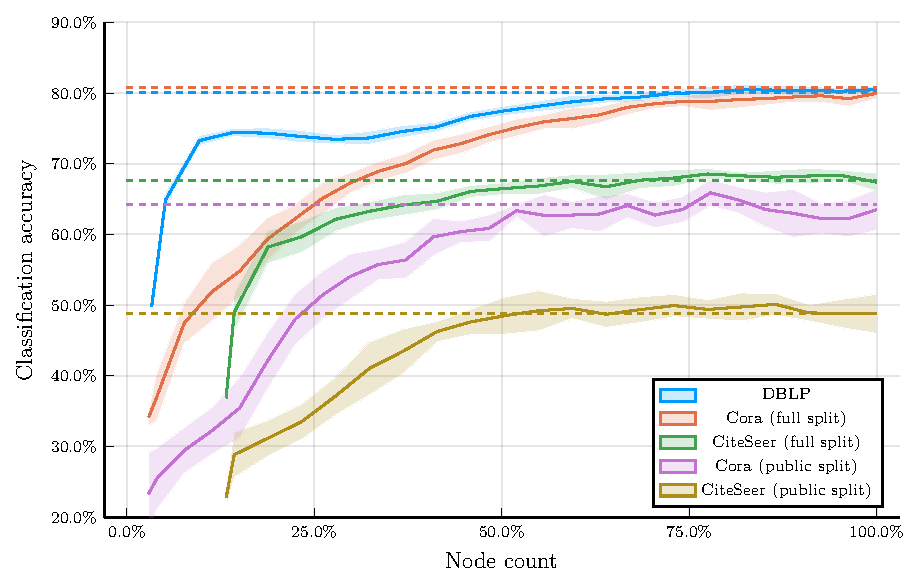
\includegraphics[width = \linewidth]{images/adaptive-coarsening/adaptive-coarsening.pdf}
  \caption{Downstream classifier accuracies at different steps of adaptive prolongation using the basic HARP coarsening algorithm. Dashed line shows the baseline node2vec model accuracy. The node count is taken relative to the total node count in each dataset. The results are averaged over multiple runs, with the solid line representing the mean and the shaded area denoting one standard deviation.}
  \label{fig:adaptive-coarsening}
\end{figure*}

The behaviour of the model somewhat differs between the used datasets. For the Cora, CiteSeer, DBLP and PubMed datasets, the model starts from a very low performance, which quickly rises as the model trains for several prolongation steps. The model trained on CiteSeer attains performance comparable to the reference model when approximately half of all nodes are available to it. On the other hand, with Cora, the model slowly approaches the reference model for the whole duration of training, only reaching comparable performance at a point where nearly the whole graph is available to it. Models trained on the two larger datasets, DBLP and PubMed, exhibit a different behaviour in that they briefly reach a global maximum followed by a slight decrease in performance until finally approaching the performance of the reference model in a manner similar to the models trained on Cora and CiteSeer. This behaviour is further discussed in the next section. The Twitch dataset is substantially different, with very high initial performance and only small performance gains with increasing number of nodes available, with different variants of it exhibiting this effect to a different magnitude.

To further study the model properties from a statistical point of view, the results were evaluated at \( k \)-th deciles of the node count of the full graph, for all possible values of \( k \). At each decile, the performance of the model was compared to the baseline node2vec model using the Wilcoxon signed-rank test with the Holm-Bonferroni correction for multiple hypothesis testing with the hypothesis that the models are equivalent. None of the hypotheses were rejected by the test at the 5\% level of significance. We attribute this mainly to the Twitch dataset, for which the performance of the adaptive approach is very good even under heavy coarsening

Following recent best-practice recommendations regarding verifying the statistical validity of results \cite{benavoli_time_2017}, the results were also studied from the point of view of Bayesian estimation. Similarly to the frequentist approach, the performance of the model was compared to that of the baseline model at \( k \)-th deciles of the node count, for all possible values of \( k \). The comparison was done using the Bayesian Wilcoxon signed-rank test \cite{benavoli_bayesian_2014} for 3 different widths of the region of practical equivalence (ROPE), 1\%, 5\% and 10\%. The probabilities that the two models are practically equivalent are listed in Table~\ref{tab:bayesian-adaptive}. Of a particular note is the fact that at 50\% complexity, the models have over a 95\% probability of being within 5 percentage points of performance -- showing that the proposed method may offer a significant complexity reduction in exchange for a relatively minor decrease in performance.

\begin{table}
  \begin{center}
    \begin{minipage}{210pt} % Tune this when the table is changed using the lua-visual-debug package
      \caption{The probabilities that the adaptive approach will be practically equivalent to node2vec when compared on different fractions of the full graph and with different widths of the region of practical equivalence.}
      \label{tab:bayesian-adaptive}
      \begin{tabular}{lrrr}
        \toprule
        \textbf{Nodes} & \textbf{1\% ROPE} & \textbf{5\% ROPE} & \textbf{10\% ROPE} \\
        \midrule
        \textbf{10\%}  & 0.1\%             & 29.1\%            & 57.8\%             \\
        \textbf{20\%}  & 0.2\%             & 39.0\%            & 90.5\%             \\
        \textbf{30\%}  & 0.1\%             & 54.5\%            & 98.6\%             \\
        \textbf{40\%}  & 0.1\%             & 71.0\%            & 100.0\%            \\
        \textbf{50\%}  & 0.9\%             & 95.2\%            & 100.0\%            \\
        \textbf{60\%}  & 8.5\%             & 99.8\%            & 100.0\%            \\
        \textbf{70\%}  & 32.6\%            & 100.0\%           & 100.0\%            \\
        \textbf{80\%}  & 62.1\%            & 100.0\%           & 100.0\%            \\
        \textbf{90\%}  & 67.4\%            & 100.0\%           & 100.0\%            \\
        \textbf{100\%} & 83.9\%            & 100.0\%           & 100.0\%            \\
        \bottomrule
      \end{tabular}
    \end{minipage}
  \end{center}
\end{table}

\subsection{The relationship of the results and the properties of the graph}

When the models for DBLP and PubMed are studied more closely, both reach a local maximum at around 14\% of the graph, followed by a slight decline and gradual approach to the baseline. This suggests a global structure in the data, which the model learns at the point of the local maxima. To investigate this hypothesis and try to explain the behaviour of the model in general, several graph metrics were applied to the graphs generated during the adaptive prolongation algorithm run. All of the metrics were applied in two scenarios -- \enquote{absolute}, where the metric was applied to the graph at a particular step in the prolongation process, and \enquote{incremental}, where the metric was applied to the graph induced by the edge set \( \mathspace{C} \), that is, the set of edges to be contracted at that step.

The metrics used were:
\begin{itemize}
  \item Edge homophily \cite{zhu_beyond_2020} is the fraction of edges connecting nodes of the same class.
  \item Node homophily \cite{pei_geom-gcn_2020} is the fraction of node neighbours having the same class as the node in question, averaged over all nodes.
  \item Class homophily \cite{lim_large_2021} is a variant of node homophily that attempts to modify it in such a way as to make it invariant to the number of classes. The metric measures excess node homophily when compared to a null model where edges are independent of node labels.
  \item Adjusted homophily \cite{platonov_characterizing_2022} is a modification of edge homophily targeted at ensuring it is not not biased towards particular class size distributions and that the metric has a constant maximum attained only for perfectly homophilous graphs.
  \item Balanced accuracy \cite{platonov_characterizing_2022} is a modification of edge homophily that balances each classes' contribution.
  \item Adjusted accuracy \cite{platonov_characterizing_2022} is a modification of balanced accuracy aimed at ensuring a constant baseline.
  \item Label informativeness \cite{platonov_characterizing_2022} is a measure of the influence of a node's neighbours' classes to the label of the node itself.
  \item Global assortativity \cite{newman_mixing_2003} is a measure of the tendency of nodes to connect with other similar nodes, rather than dissimilar nodes.
\end{itemize}

The values of these metrics at different steps of the adaptive prolongation algorithm are shown in Figure~\ref{fig:metrics-absolute} and Figure~\ref{fig:metrics-incremental}. In both the absolute and incremental scenarios, most metrics rise over training until hitting a plateau at the same point as the performance stop increasing. The change is the most pronounced in the global assortativity metric, which actually decreases after this point. This suggests the explanation of the graphs being heterophilic when very coarse (as could be expected), then reaching a point where the global structure of the graph is in place and is then only refined in a local sense. Such a behaviour may introduce nodes which have a different label than their neighbourhoods (a kind of noise in the data), which is a possible explanation for the local minimum in performance.

\begin{figure*}
  \centering
  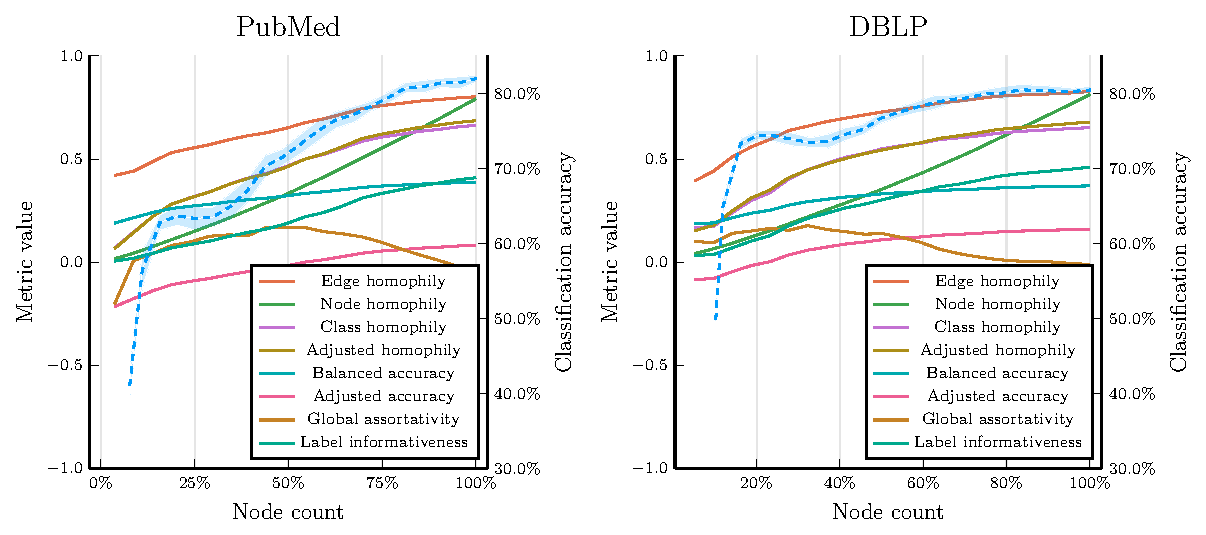
\includegraphics[width = \linewidth]{images/metrics-absolute/metrics-absolute.pdf}
  \caption{Values of the metrics for different datasets at different steps of the adpative prolongation algorithm in the absolute scenario. Overlaid as the dashed line is the accuracy of the downstream classifier.}
  \label{fig:metrics-absolute}
\end{figure*}

\begin{figure*}
  \centering
  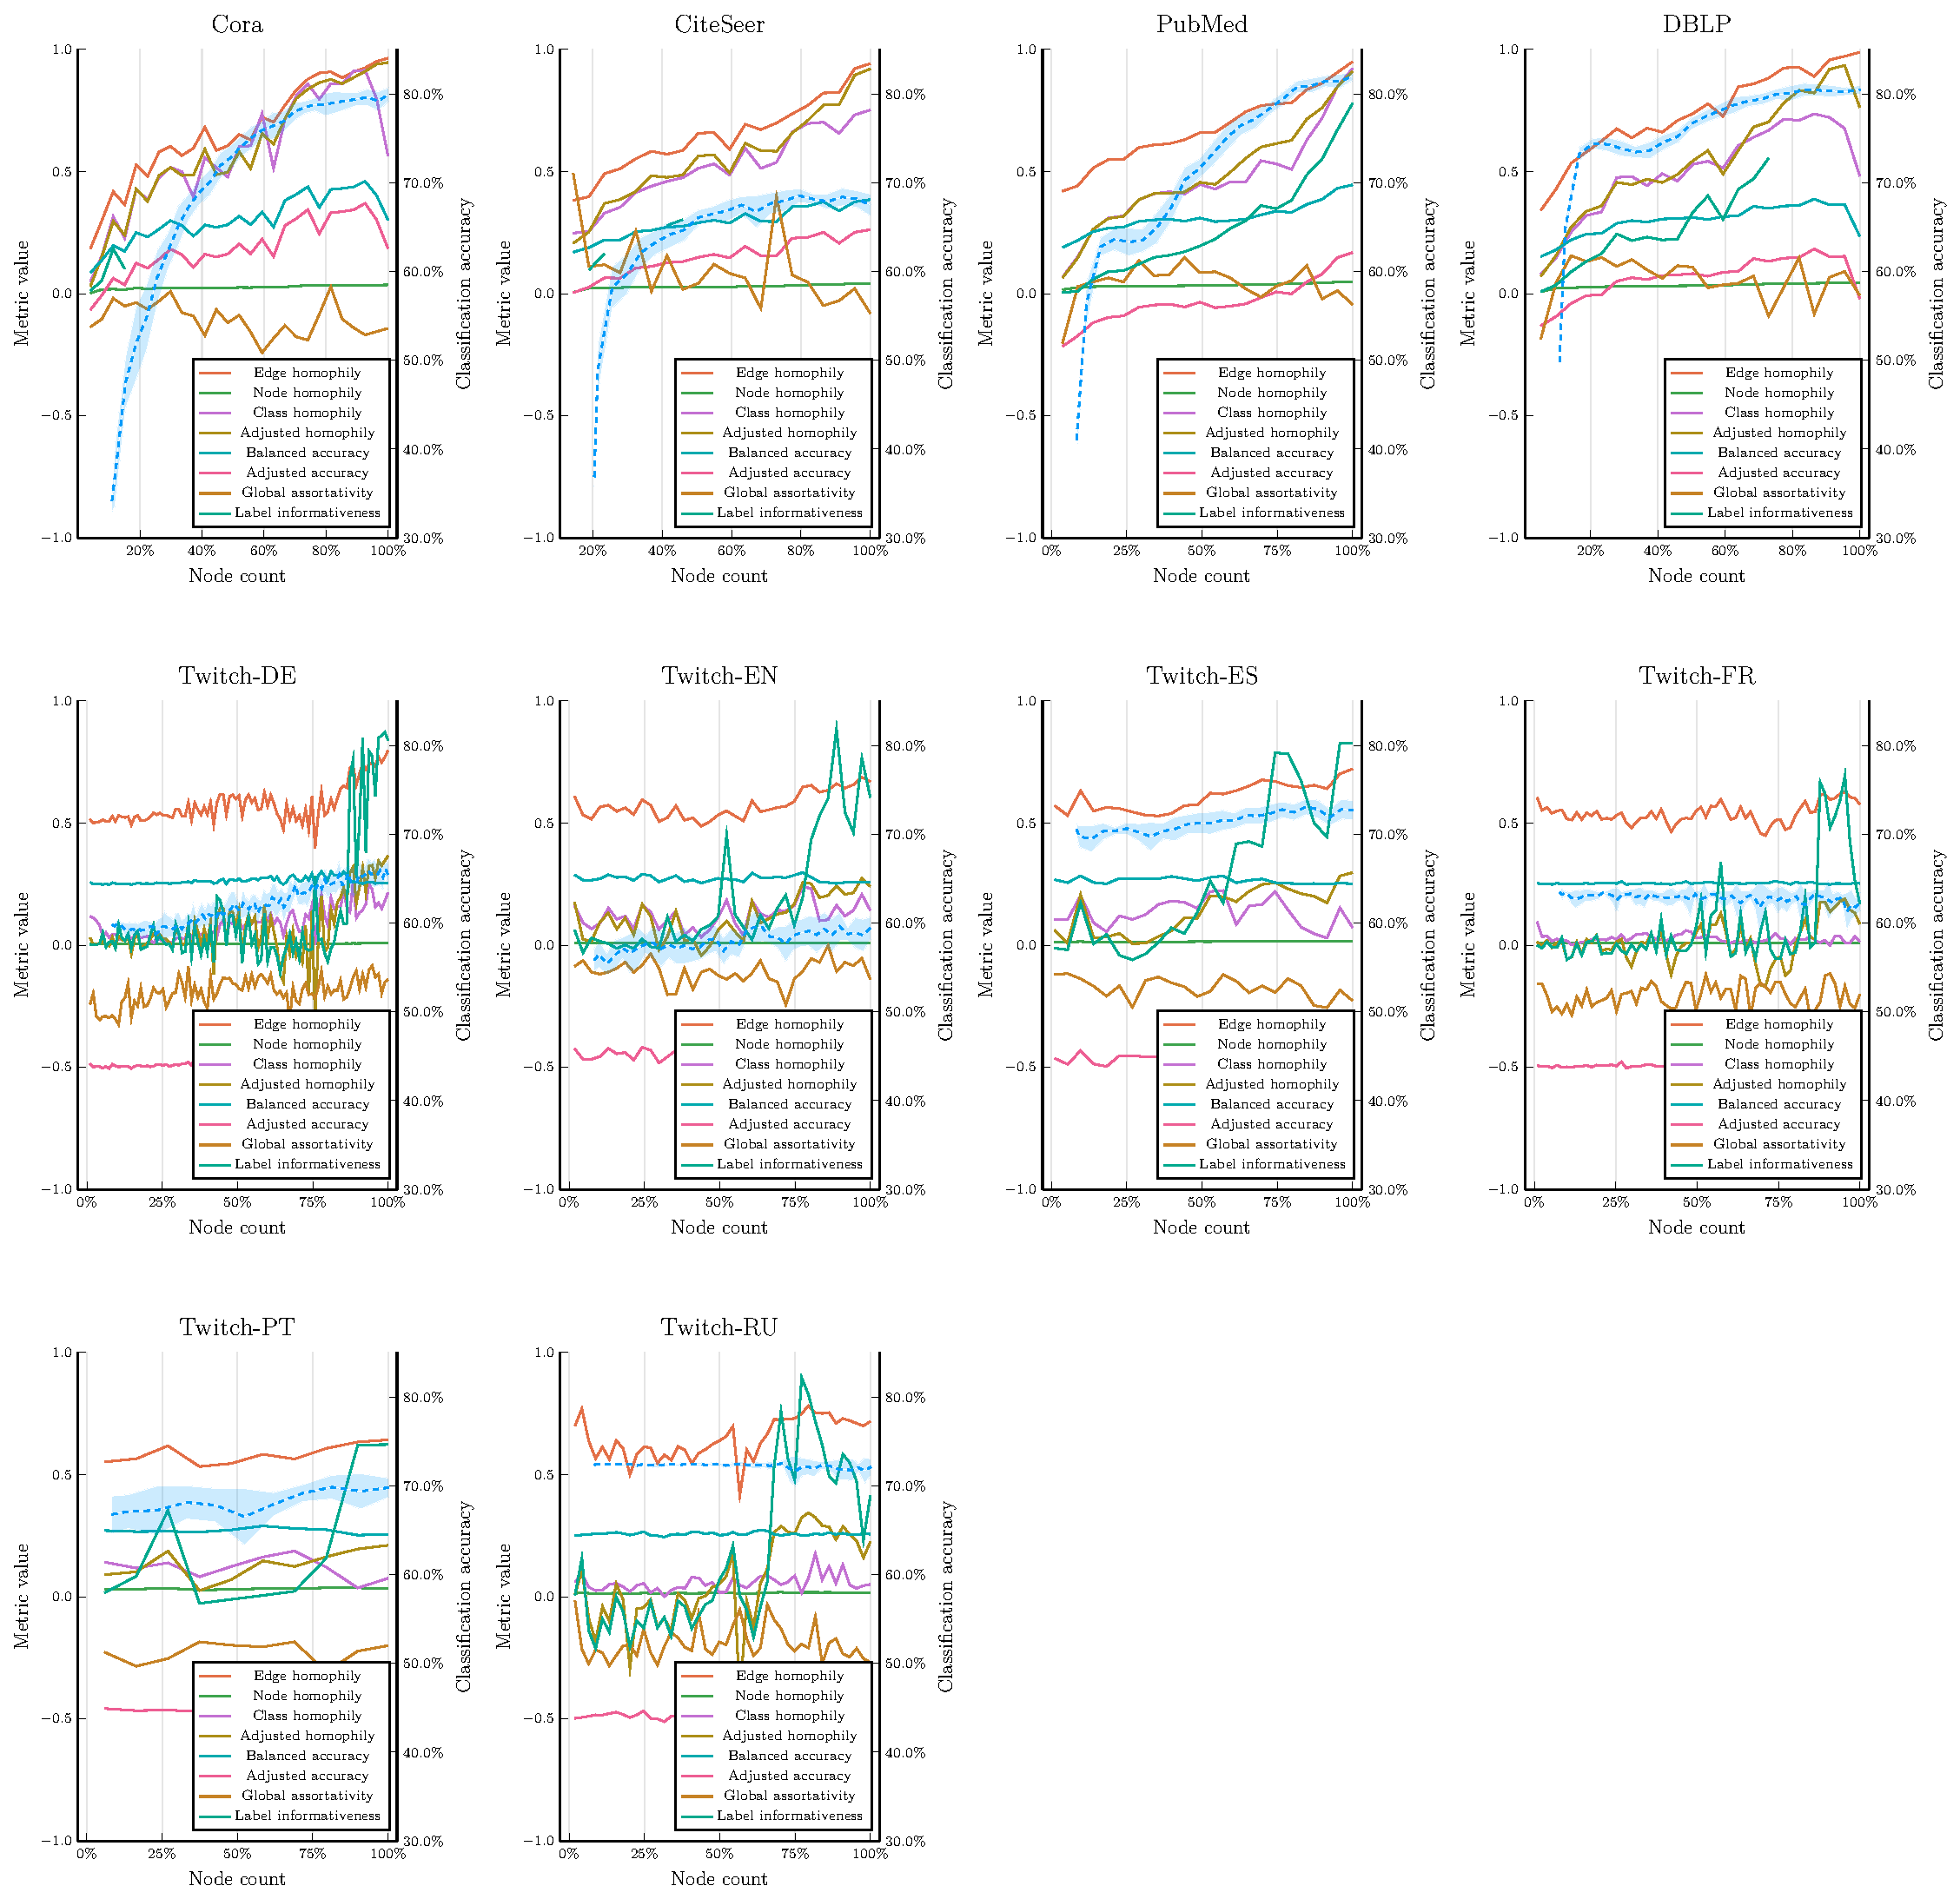
\includegraphics[width = \linewidth]{images/metrics-incremental/metrics-incremental.pdf}
  \caption{Values of the metrics for different datasets at different steps of the adpative prolongation algorithm in the incremental scenario. Overlaid as the dashed line is the accuracy of the downstream classifier.}
  \label{fig:metrics-incremental}
\end{figure*}

\subsection{Comparison of coarsening approaches}

For GDC coarsening, only the top-\( k \) sparsification method produces reliable results as thresholding leads to instability in the coarsening process, either collapsing the whole graph almost immediately, or not collapsing it at all. As for the other parameters, we followed \cite{gasteiger_diffusion_2019}. Both of the diffusion methods propsed in \cite{gasteiger_diffusion_2019} were implemented with the recommended parameter values, that is the heat kernel was used with the diffusion time \( t = 5 \) and the Personalized PageRank algorithm with the teleport probability \( \alpha = 0.15 \) and the recommended normalization. To be able to compute graph diffusion for larger graphs, approximate diffusion algorithms were used. For PPR, a version of the Andersen algorithm \cite{andersen_local_2006} with \( \epsilon = 10^{-2} \) was used and for heat kernel diffusion, a version of the Kloster-Gleich algorithm \cite{kloster_heat_2014} with \( \epsilon = 10^{-5} \) was used. Both of these algorithms were modified to produce edge weights as part of their output.

\begin{figure*}
  \centering
  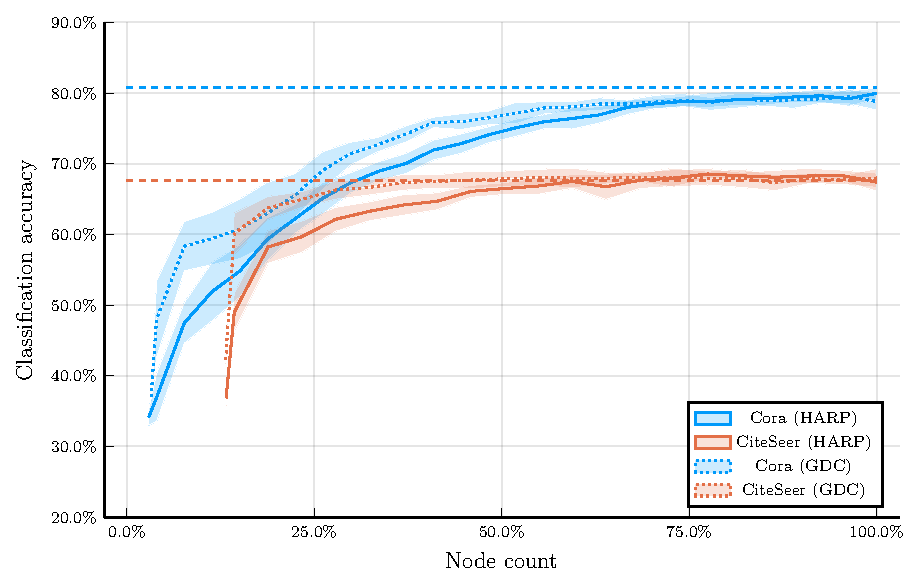
\includegraphics[width=\linewidth]{images/coarsening-algorithms/coarsening-algorithms.pdf}
  \caption{Downstream classifier accuracies at different steps of adaptive prolongation for different coarsening algorithms. Dashed line shows the baseline node2vec model accuracy. The node count is taken relative to the total node count in each dataset. The results are averaged over multiple runs, with the solid line representing the mean and the shaded area denoting one standard deviation.}
  \label{fig:coarsening-algorithms}
\end{figure*}

The behaviour of the models (Figure~\ref{fig:coarsening-algorithms}) again differs substantially between the datasets. Generally, the methods behave in a similar manner, retaining decent performance even at coarser levels and only improving slightly as more data is available. For Cora, CiteSeer, PubMed and DBLP datasets, the GDC based coarsenings outperform standard HARP at most coarsening levels, with PPR having higher accuracy when there is a difference between the two. This suggests that the GDC algorithm is able to preserve the global structure of the graph better than HARP over successive coarsenings. Twitch-EN and Twitch-PT are the only two datasets where HARP outperforms the diffusion-based methods, with other variants showing either comparable performance of all the approaches, or a preference towards GDC. Of note is the fact that the PPR algorithm only coarsened some variants of the Twitch dataset slightly, a problem not shared by the heat diffusion approach.

Statistical tests similar to the ones described in Section~\ref{sec:adaptive-experiments} were carried out to compare the different models. The Friedmann two-way analysis of ranks with the Holm-Bonferroni correction was used to test the hypothesis that all of the methods are equivalent at \( k \)-th deciles for all possible values of \( k \). This hypothesis was rejected for \( k \in \left\{ 1, 2, 3, 4 \right\} \) with Holm-corrected familywise p-values \( 3.36 \times 10^{-3}, 4.35 \times 10^{-3}, 7.36 \times 10^{-4}, 6.77 \times 10^{-3} \), respectively. For these deciles, a post-hoc pairwise Wilcoxon test was performed between the HARP, PPR and heat kernel methods. At the 5\% significance level, the test did not reject the hypothesis that HARP and the heat kernel are equivalent for any \( k \), rejected the hypothesis that HARP and PPR are equivalent for all values of \( k \in \left\{ 1, 2, 3, 4 \right\} \) with Holm-corrected p-values \( 0.023, 0.023, 0.023, 0.047 \) respectively and rejected the hypothesis that the heat kernel and PPR are equivalent for \( k \in \left\{ 1, 3 \right\} \) with Holm-corrected p-values \( 0.035, 0.046 \) respectively.

The coarsening approaches were also compared using Bayesian estimation, using the Bayesian Wilcoxon signed-rank test in a pairwise fashion for all possible values of \( k \) with a 5\% region of practically equivalence. When comparing HARP to the heat kernel, the two methods had over 98\% probability of being practically equivalent for all values of \( k \). The comparison of HARP and PPR is listed in Table~\ref{tab:bayesian-harp-ppr} and the comparison of the heat kernel and PPR in Table~\ref{tab:bayesian-heat-ppr} The results show that all the methods are practically equivalent when the graph is only slightly coarsened and at higher levels of coarsening, PPR dominates both other methods in the situations where it is available.

\begin{table}
  \begin{center}
    \begin{minipage}{180pt} % Tune this when the table is changed using the lua-visual-debug package
      \caption{Comparison of HARP coarsening and PPR based coarsening based on the Bayesian Wilcoxon signed-rank test. The left an right columns list the probability of each respective method having higher accuracy, while the middle column shows the probability of the 2 methods being practically equivalent with a 5\% ROPE.}
      \label{tab:bayesian-harp-ppr}
      \begin{tabular}{lrrr}
        \toprule
        \textbf{Nodes} & \textbf{HARP} & \textbf{Equivalent} & \textbf{PPR} \\
        \midrule
        \textbf{10\%}  & 0.0\%         & 41.1\%            & 58.9\%         \\
        \textbf{20\%}  & 0.0\%         & 69.1\%            & 30.9\%         \\
        \textbf{30\%}  & 0.0\%         & 84.5\%            & 15.5\%         \\
        \textbf{40\%}  & 0.0\%         & 97.9\%            & 2.2\%          \\
        \textbf{50\%}  & 0.0\%         & 99.8\%            & 0.2\%          \\
        \textbf{60\%}  & 0.0\%         & 100.0\%           & 0.0\%          \\
        \textbf{70\%}  & 0.0\%         & 100.0\%           & 0.0\%          \\
        \textbf{80\%}  & 0.0\%         & 100.0\%           & 0.0\%          \\
        \textbf{90\%}  & 0.0\%         & 100.0\%           & 0.0\%          \\
        \textbf{100\%} & 0.0\%         & 100.0\%           & 0.0\%          \\
        \bottomrule
      \end{tabular}
    \end{minipage}
  \end{center}
\end{table}

\begin{table}
  \begin{center}
    \begin{minipage}{180pt} % Tune this when the table is changed using the lua-visual-debug package
      \caption{Comparison of heat kernel and PPR based coarsenings based on the Bayesian Wilcoxon signed-rank test. The left an right columns list the probability of each respective method having higher accuracy, while the middle column shows the probability of the 2 methods being practically equivalent with a 5\% ROPE.}
      \label{tab:bayesian-heat-ppr}
      \begin{tabular}{lrrr}
        \toprule
        \textbf{Nodes} & \textbf{Heat} & \textbf{Equivalent} & \textbf{PPR} \\
        \midrule
        \textbf{10\%}  & 0.0\%         & 58.1\%            & 41.9\%         \\
        \textbf{20\%}  & 0.0\%         & 89.4\%            & 10.6\%         \\
        \textbf{30\%}  & 0.0\%         & 99.9\%            & 0.1\%         \\
        \textbf{40\%}  & 0.0\%         & 100.0\%           & 0.0\%          \\
        \textbf{50\%}  & 0.0\%         & 100.0\%           & 0.0\%          \\
        \textbf{60\%}  & 0.0\%         & 100.0\%           & 0.0\%          \\
        \textbf{70\%}  & 0.0\%         & 100.0\%           & 0.0\%          \\
        \textbf{80\%}  & 0.0\%         & 100.0\%           & 0.0\%          \\
        \textbf{90\%}  & 0.0\%         & 100.0\%           & 0.0\%          \\
        \textbf{100\%} & 0.0\%         & 100.0\%           & 0.0\%          \\
        \bottomrule
      \end{tabular}
    \end{minipage}
  \end{center}
\end{table}
